\section{Methods and Materials}
\label{sec:coronary_methods}

This section outlines the work flow of the segmentation and presents the mathematical principles of the consisting modules.
The work flow of the segmentation process is illustrated in the bird's-eye view (see Figure \ref{fig:coronary_data_flow}).
Since our work is concentrated on the heart area, i.e., the coronary arteries in this paper, the region of interest (ROI) in the original CTA slices were completely extracted, right before all other processing. %
To make the following level set evolution generate a better result, the noisy pixels are depressed without affecting the edges of the vasculature.
Then the images are appropriately thresholded, stripping off the contents irrelevant to our mission.
Two computations to generate the image features and the initial contours for the CURVES system are triggered simultaneously.
The image features are calculated on the gradient maps which are shaped by the gradient magnitude module.
On the other hand, the threholded images are sent to the fast marching module to evolve the initial contour.
After that, both the results are transferred to the CURVES module in order to segment the boundaries of the vasculature.
In the end, the resulting level sets are thoroughly extracted to form the surface model information.
\begin{figure}[tb]
\centering
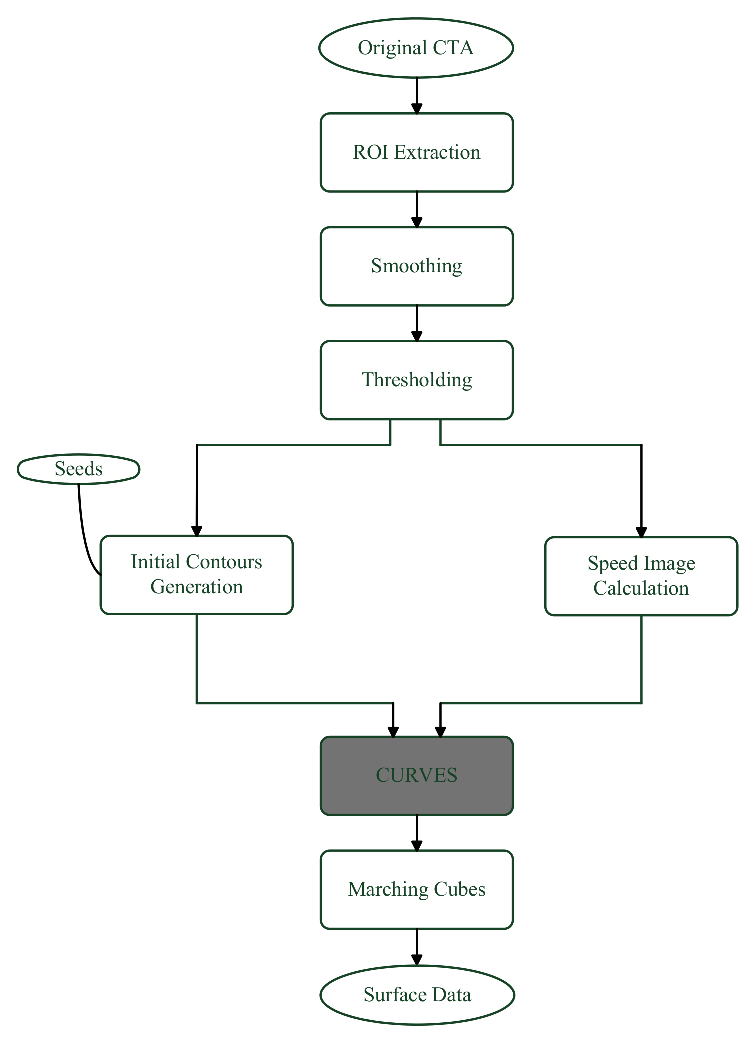
\includegraphics[width=3.2in]{Figures/coronary/DataFlow}
\caption{Flowchart of the segmentation pipeline.}
\label{fig:coronary_data_flow}
\end{figure}

\subsection{Preprocessing for Fronts Evolution}
\label{subsec:coronary_preprocessing}

\subsubsection{Image Conditioning for Further Processing}
\label{subsubsec:coronary_condition}

In the raw images directly acquired from the medical modalities, noisy pixels unavoidably exist, which makes smoothing a necessary step before any further operation.
Hence, after fully extracted the ``heart" from the original images, the next concern is to smooth these noisy pixels without significantly affecting the boundaries of the vasculature. %
Bear this in mind, the level-set curvature method with variable conductance \cite{Whitaker2001} is chosen for this job for two reasons: (1) this method is good at preserving edges; and (2) this method is robust to the edge contrast.
%\begin{itemize}
%\item this method is good at preserving edges;
%\item this method is robust to the edge contrast.
%\end{itemize}
According to paper \cite{Whitaker2001}, the method can be described as the following modified curvature diffusion equation:
\begin{equation}
\label{eqn:coronary_MCDE}
I_t = |\nabla I| \nabla \cdot c(|\nabla I|) \frac{\nabla I}{|\nabla I|},
\end{equation}
where $I$ denotes the image, and $c$ is the conductance function. %

After the smoothing step, a general threshold filter is employed to remove the image contents that are unrelated to the segmentation.
Concretely, the intensities lie between the interval specified by the lower and upper thresholds remain the same whilst the intensities beyond this interval are set to zero value. %

\subsubsection{Speed Images Calculation}
\label{subsubsec:coronary_speed_image}

Level set evolution relies on the gradient field as its guidance, in which the steep variations in intensities from the inner or outer area to the edges indicate the evolution a halt signal.
The calculation is performed on the thresholded image series containing the targeting objects.
In calculating the image features, the first task is to compute the magnitudes of gradients pixel-wisely to produce a gradient field map.
Here, the Gaussian kernel is adopted as the convolution kernel in calculating the gradients.

Next, the gradient images $I_{\nabla}$ are transformed into the speed images $I_{\sigma}$ by applying the nonlinear function:
\begin{equation}
\label{eqn:coronary_sigmoid}
I_{\sigma} = \frac{I_{max} - I_{min}}{1 + \exp\left(-\frac{I_{\nabla} - n}{m}\right)} + I_{min},
\end{equation}
where $I_{max}$ and $I_{min}$ are the maximum and minimum of the output intensity values in the output image $I_{\sigma}$, respectively; $m$ is a constant specifies the range of the input intensity, and $n$ is a constant controls the center of the range.

\subsubsection{Initial Contours Generation}
\label{subsubsec:coronary_initial_contours}

The fast marching algorithm \cite{Sethian1999} is employed to fulfill the task of generating the initial level sets required by the CURVES system.
The algorithm starts the evolution from several seeding points (seeds) within the areas representing the targets provided by the user.
Then the contours surrounding each seed propagate ``outwards" until they meet the boundaries of the targets.
This is equivalent to solving the Eikonal equation in \cite{Sethian1999}: $1 = | \nabla T | F$, %
%\begin{equation}
%1 = | \nabla T | F,
%\end{equation}
where $F$ is the velocity in the normal direction at some point $(x,y)$ in the image.
The evolving curve $\mathcal{C}$ is defined as $\mathcal{C}(t) = \{(x,y) | T(x,y) = t\}$, %
%\begin{equation}
%\label{eqn:coronary_Curves}
%\mathcal{C}(t) = \{(x,y) | T(x,y) = t\},
%\end{equation}
where $T(x,y)$ is the time-of-arrival function.
$\mathcal{C}$ evolves over time $t$: it propagates ``inwards" when $F < 0$; it propagates ``outwards" when $F > 0$.
On the termination of the propagation, the map of the time-of-arrival of the contour is given.
This mechanism demonstrates its advantage in generating the initial level sets of the prolonged targets for the main level set system.

\subsection{CURVES Model}
\label{subsec:coronary_CURVES}

As the candidate method for the effort of the three dimensional segmentation of the coronary arteries tree structure, the CURVES system \cite{Lorigo2001} is highly effective in extracting the complex spatial curvilinear structures in the volumetric data.
Moreover, the CURVES's criterion also takes the local smoothness of the edges to be detected (i.e., the inner wall of the coronary arteries) into consideration.

As the extension of the geodesic active contours \cite{Caselles1997}, CURVES is a level set algorithm that models the vasculature as spatial curves with arbitrarily complicated topology \cite{Lorigo2001}. %
The algorithm evolves the level sets from the initial contours to the boundaries of the targets subjected to the minimization of the functional
\begin{equation}
\label{eqn:coronary_CURVES}
\oint_0^1 g\left( \left| \nabla I \left( \mathcal{C} \left(  s \right) \right) \right| \right) \left| \mathcal{C}'\left( s \right) \right| ds,
\end{equation}
where $\mathcal{C}: [0,1] \rightarrow \mathrm{R}^3$ is a spatial curve, $I: [0, a] \times [0, b] \times [0, c] \rightarrow [0, \infty)$ is the input image, and $g: [0, \infty) \rightarrow \mathrm{R}^+$ is a monotonically decreasing function. %

The minimum of the functional can be found by searching for the gradient descent direction of the functional per se, which means the Euler-Lagrange equations of (\ref{eqn:coronary_CURVES}) must be solved. %
Then the geodesic flow equation that regulates the propagation can be obtained as follows
\begin{equation}
\label{eqn:coronary_evolution}
\frac{\partial \mathcal{C}}{\partial t} = k \mathcal{N} - \frac{g'}{g} \varPi \left( \mathcal{H} \frac{\nabla I}{ \left| \nabla I \right| } \right),
\end{equation}
where $\mathcal{H}$ is the Hessian matrix of the input image $I$, $\mathcal{N}$ is the unit normal, $k$ is the curvature, $\varPi$ is the projection operator projects the arguments onto the normal space. %
%The update equation can be obtained as
%\begin{equation}
%\label{eqn:Update}
%\frac{\partial v}{\partial t} = \mathcal{F} \left( \nabla v(x, t), \nabla^2 v(x, t) \right) + \frac{g'}{g} \nabla v(x, t) \mathcal{H} \frac{\nabla I}{ \left| \nabla I \right| },
%\end{equation}
%where $v(\cdot): \mathrm{R}^3 \rightarrow [0, \infty)$ is the embedding function of the curve $\mathcal{C}$, $\mathcal{F} \left( \nabla v(x, t), \nabla^2 v(x, t) \right)$ is the smaller eigenvalue of the matrix $P_{\nabla v} \nabla^2 v P_{\nabla v}$. %
%The matrix $P_q$ is defined as a projector which projects some vector onto the normal plane of vector $q \in \mathrm{R}^3$:
%\begin{equation}
%\label{eqn:ProjectionOperator}
%P_q = I_0 - \frac{qq^T}{\left| q \right|^2},
%\end{equation}
%where $I_0$ denotes the identity matrix.

By substituting the input image $I$ with the speed image $I_{\sigma}$ generated by (\ref{eqn:coronary_sigmoid}) to the evolution equation (\ref{eqn:coronary_evolution}), the evolution equation can be written as
\begin{equation}
\label{eqn:coronary_application}
\frac{\partial \mathcal{C}}{\partial t} = k \mathcal{N} - \frac{g'(I_{\sigma})}{g(I_{\sigma})} \varPi \left( \mathcal{H} \frac{\nabla I_{\sigma}}{ \left| \nabla I_{\sigma} \right| } \right).%
\end{equation}
Observing (\ref{eqn:coronary_application}), the contour evolution is restricted by the three factors: (1) the image features, (2) the force driving the contour ``inwards" or ``outwards", and (3) the curvature minimization.

\subsection{Surface Extraction}
\label{coronary_surface_extraction}

The surface information is extracted for the final visualization by the marching cubes method \cite{Lorensen1987MC}.
Cubes are created based on the input information and are organized into an array structure.
Each of them consists of eight pixels, with each four from the same slice.
The indices of the cubes are marked with the information generated by comparing the intensities of each vertex to the isovalue of the surfaces.
Next the intersection between surfaces and cubes are roughly figured out based on the classic 14 triangulated cases.
After that, the accurate intersection location are calculated by applying linear interpolation with the pixel intensities of each vertex.
The central differences method is applied on the vertices of the cubes in order to calculate the unit normals to the surfaces.
Finally the resulting polygons are organized and prepared for the surface rendering performed by the graphics hardware.
